\documentclass[../../main.tex]{subfiles}
\graphicspath{{images/imagesPREN1/}{../../images/imagesPREN1/}}
\begin{document}
\subsection{Würfelaufnahme}
\subsection{Würfelaufnahme/Transport}
         Um den Würfel rechts neben der Gleisstrecke aufzunehmen, wird eine einfache Lösung angestrebt, steuerungstechnisch sowie mechanisch. Aus dem morphologischen Kasten (Anhang) und der Nutzwertanalyse geht hervor, dass die Würfelaufnahme mit einem Draht und einem Stab durchgeführt wird. Damit nur ein Aktor angesteuert werden muss, wird von dem Prinzip einer Kurvenscheibe Gebrauch gemacht. Die gesamte Vorrichtung besteht grundsätzlich aus drei Elementen: Einem Kran zur Lastaufnahme, einem Antriebsstrang und der Kurvenscheibe.

        \begin{figure}[H]
            \centering
            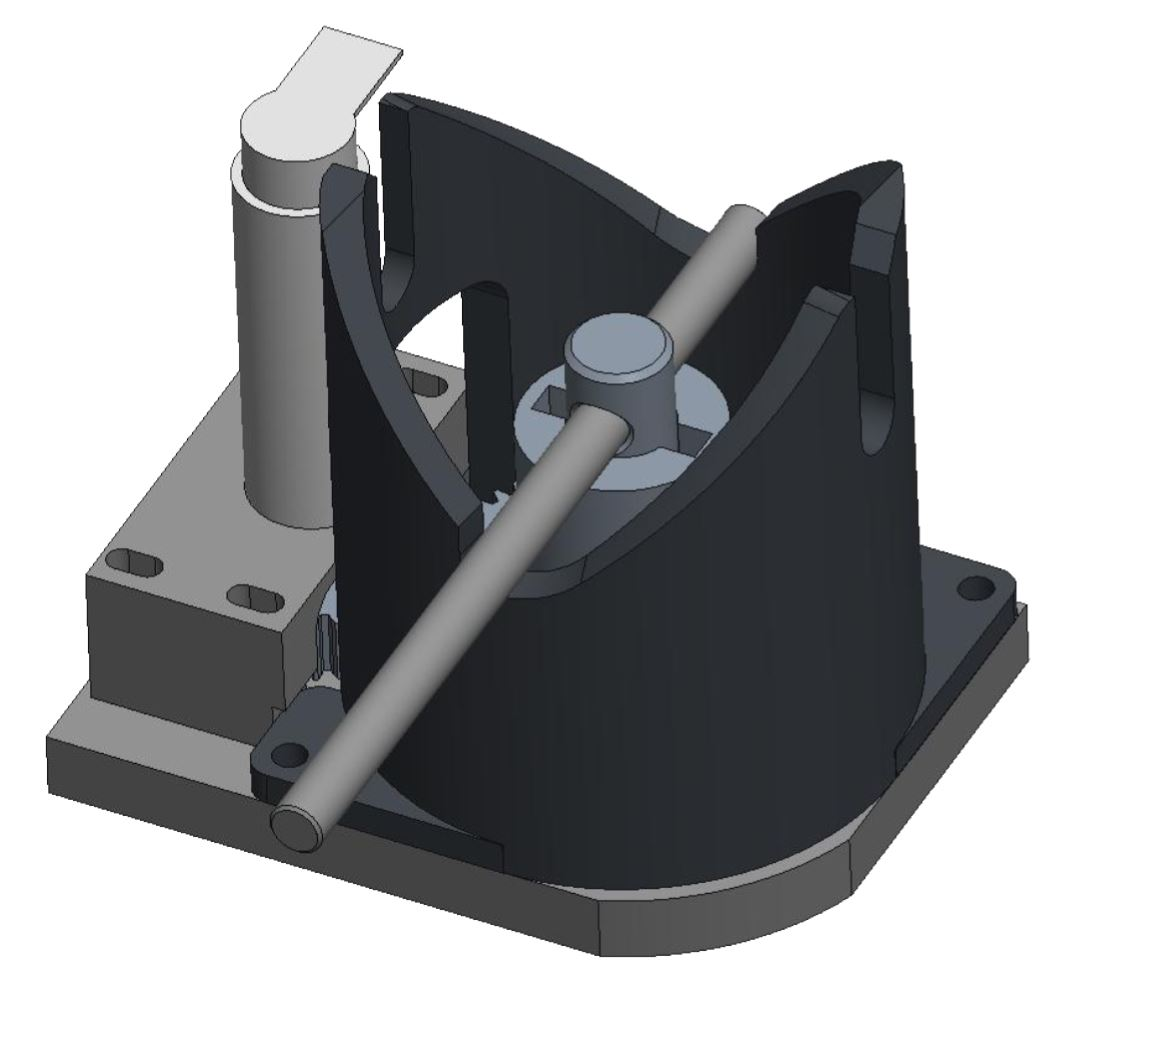
\includegraphics[width=0.5\textwidth]{Kran/BG_3.JPG}
            \caption {Baugruppe}
        \end{figure}

    \subsubsection{Kran}
         Der Kran besteht aus drei Drehteilen, welche mit einer Pressverbindung zusammengefügt wurden. Das zentrale Element des Krans wird auf Grund seiner optimalen Gleiteigenschaften und der geringen Dichte aus Teflon gefertigt. Der kleinere Stahlstift ist für die Drehmomentübertragung zuständig. Der grössere der beiden Stahlstifte ist der eigentliche Ausleger. An dessen Ende wird ein Draht aus Federstahl geformt und angehängt. Dieser Draht soll als Haken zur Lastaufnahme dienen. Weiter ist der Ausleger in beide Richtungen von der Drehachse ausgedehnt, da die Kurvenscheibe zwei Laufflächen hat, um für einen stabilen Hub zu sorgen. Der ganze Aufbau wird mittels einer Spielpassung in einer Bohrung mit zwei Längsnuten in einem 3D gedruckten, modifizierten Zahnrad gelagert.

        \begin{figure}[H]
            \centering
            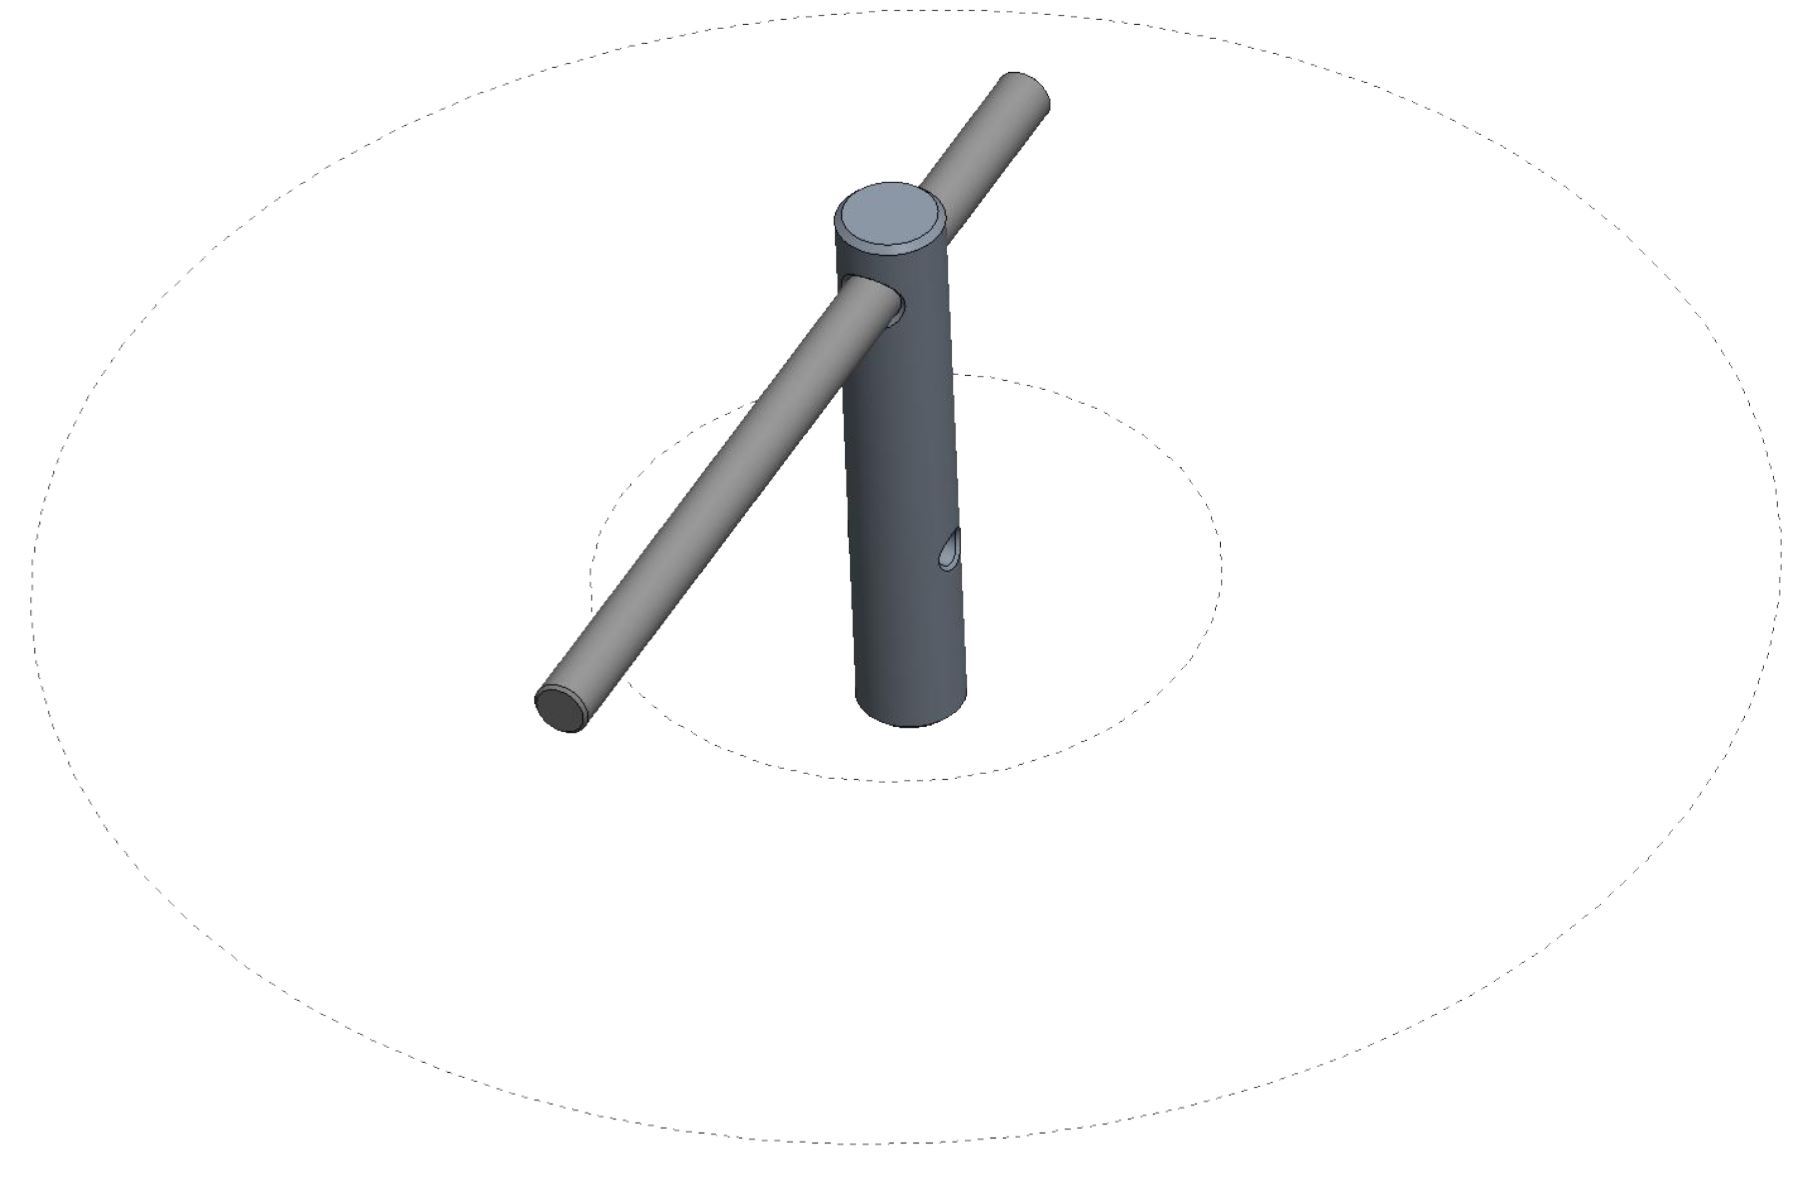
\includegraphics[width=0.4\textwidth]{Kran/Top_3.JPG}
            \caption {Draufsicht}
        \end{figure}



    \subsubsection{Antriebsstrang}
        Der Antrieb besteht aus einem Motor, dessen Aufhängung und zwei Zahnrädern. Der Motor ist ein bürstenbehafteter
        Motor mit Encoder und Getriebe vorne drauf. Mit dieser Variante und der Übersetzung, zusammengesetzt aus Getriebe
        und Zahnrädern, kann von der Steuerung aus genau definiert werden, wie viele Umdrehungen der Motor benötigt, um
        mit dem Kranausleger eine Viertelumdrehung zu fahren. Das eine Zahnrad ist Standard und von Mädler eingekauft.
        Das zweite Zahnrad jedoch wurde nur als STEP von Mädler heruntergeladen und anschliessend im CAD bearbeitet. Die
        Bohrung und der Flansch in der Mitte wurden verlängert und mit zwei Längsnuten versehen. Die Bohrung gilt als
        Axialführung und die Nuten dienen als Drehmomentübertragung.


        \subsubsection{Kurvenscheibe}
        Die Kurvenscheibe ist ebenfalls ein 3D-Druckteil. Der Grundkörper ist ein Rohr mit dem Aussendurchmesser 80 mm. An diesem wurden zwei Bahnführungen mittels Freiformflächen für den Kranausleger erzeugt. Die Steigung dieser Flächen ist variabel. Zu Beginn ist die Steigung gering und wird dann exponentiell grösser. Dies wurde aus dem einen Grund gewählt, damit das Anfahren für den Motor nicht zu streng ist. Nachdem die Drehbewegung und der vertikale Hub gemacht wurden, stoppt der Motor und der Kranausleger sollte durch die Schwerkraft heruntergezogen werden. Der Würfel wird nun in der für ihn vorgesehenen Aufnahme auf dem Zug platziert.\\


        \begin{figure}[H]
            \centering
            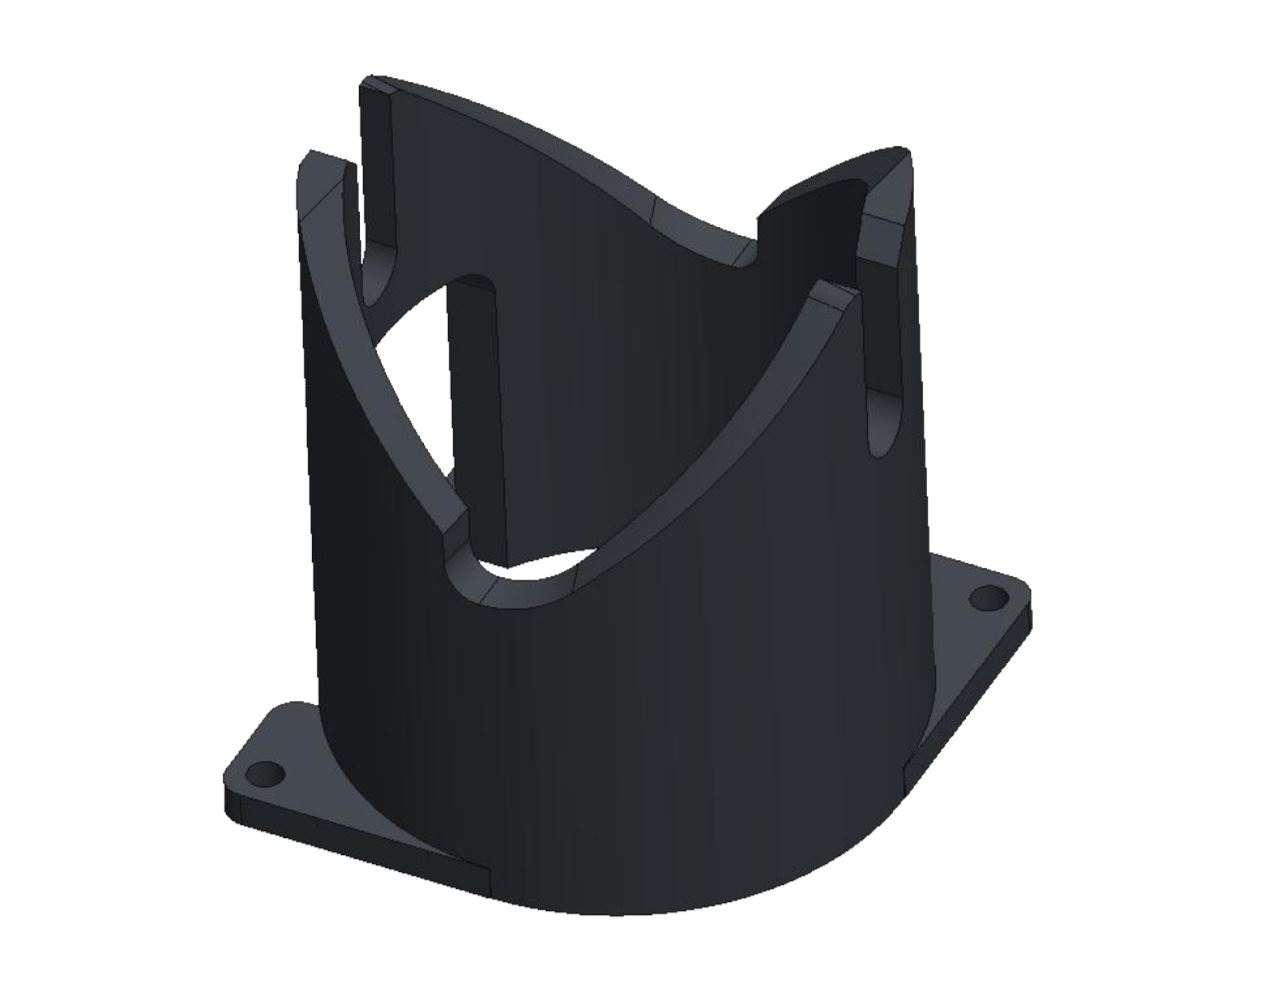
\includegraphics[width=0.6\textwidth]{Kran/Kurvenscheibe_3.JPG}
            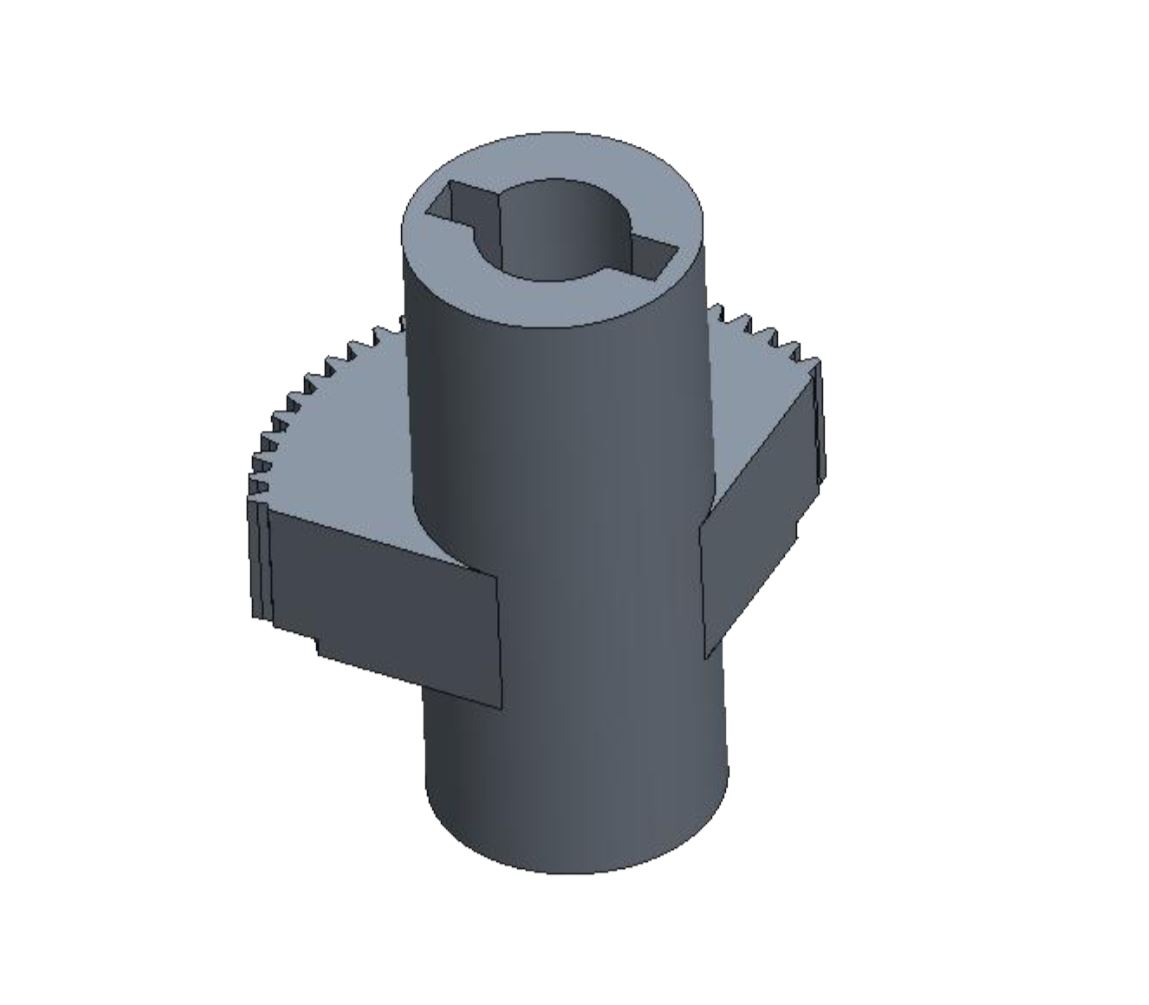
\includegraphics[width=0.35\textwidth]{Kran/Zahnrad_3.JPG}
            \caption {Links: Kurvenscheibe,  Rechts: Zahnrad}
        \end{figure}
        \pagebreak


        \subsubsection{Testaufbau}
        Der Testaufbau besteht hauptsächlich aus 3D-Druckteilen und weichen Kunststoffen. Er dient momentan als Funktionsmuster. Wenn sich dieser weiter bewährt, möchte man mit den gefertigten Teilen weiterarbeiten. Der Test dient zur Probe des ausgewählten Lösungskonzepts der Würfelaufnahme. Erste Tests zeigen, dass die Funktion mit kleinen Anpassungen direkt umgesetzt werden kann.

        \begin{figure}[H]
            \centering
            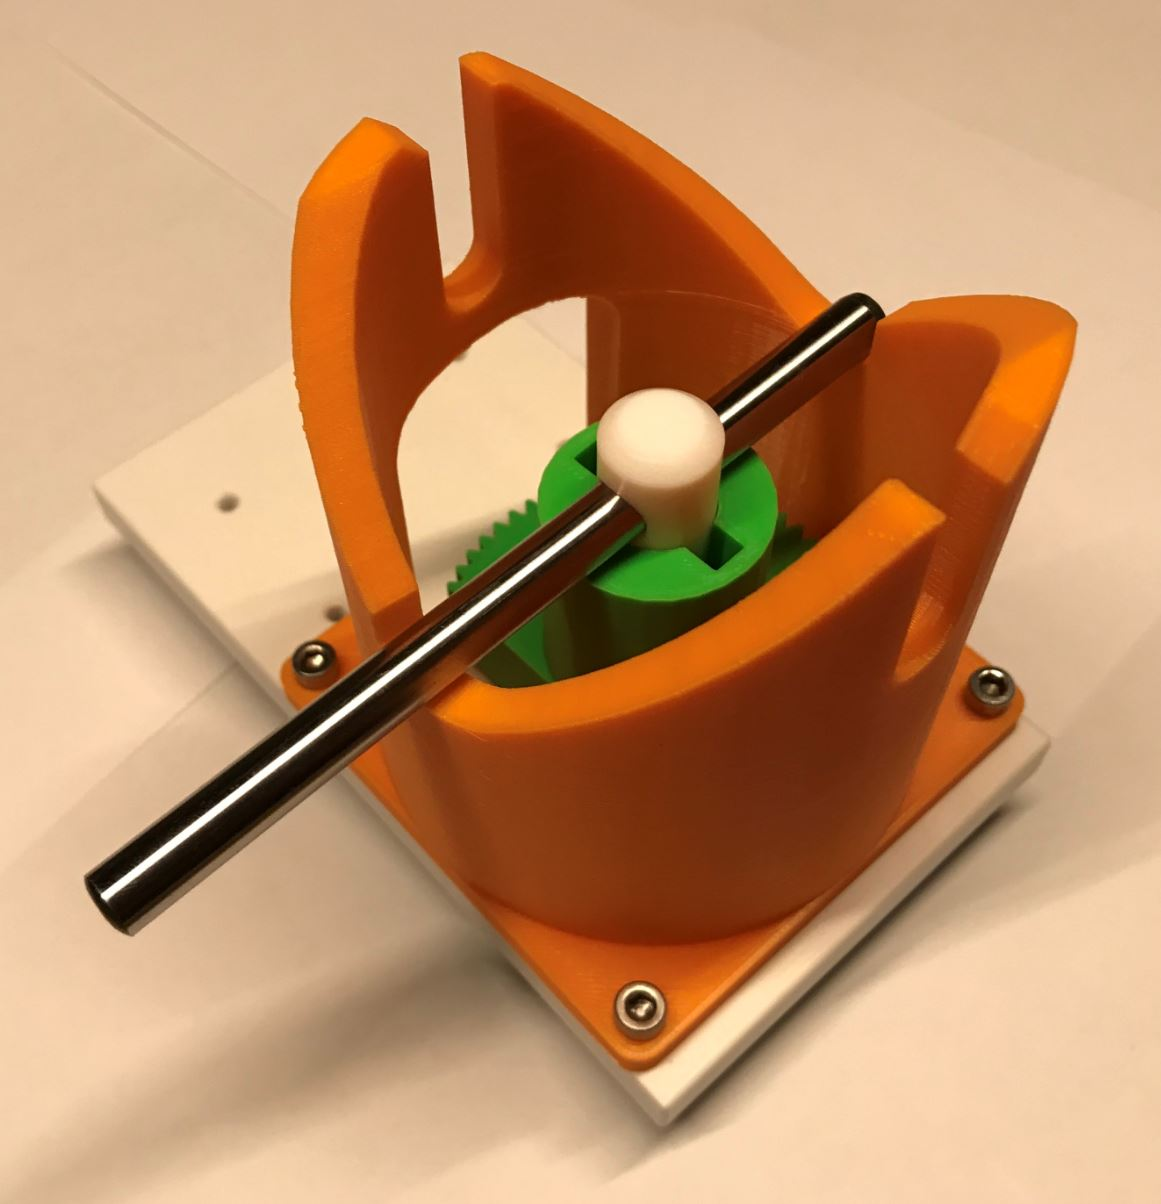
\includegraphics[width=0.8\textwidth]{Kran/Testaufbau.JPG}
            \caption {Testaufbau}
        \end{figure}
        \pagebreak


    \subsection{Motorauslegung}
          Um die Aufgabenstellung der schnellen Fahrt auf Schienen bestmöglichst zu erfüllen, wird ein zuverlässiger
          starker Motor benötigt. Um einen solchen aus einer Vielzahl von Auswahlmöglichkeiten zu definieren, hat man
          sich auf den Katalog definiert maxon motor ag beschränkt. Im Anhang findet man ein Dokument mit den
          Berechnungen zur Motorauswahl. In Absprache der Disziplinen Elektrotechnik und Maschinentechnik wurde ein
          bürstenbehafteter Gleichstrommotor als geeignetes Modell definiert. Im vorher schon erwähnten Dokument wird für
          den gesamten Zug eine Masse von 3 Kilogramm gerechnet und einen Raddurchmesser von 22 mm. Für eine
          Endgeschwindigkeit von 3 m/s mit den definierten Raddurchmessern ergibt sich eine Drehzahl von 2600 1/min. Mit
          einer Übersetzung von 2, was mit Zahnrädern und den Platzverhältnissen gut realisierbar ist, ergibt sich eine
          Abgangsdrehzahl für den Motor von 5200 1/min. Das ist im Rahmen der Motoren von maxon motor ag. Was jedoch den
          Motor an seine Grenzen führt, wird die Grenzbeschleunigung sein. Durch die Beschleunigung bedingte
          Trägheitskraft, welche durch ein Moment vom Motor überwunden werden muss. Das Moment rechnet sich aus der
          gewollten Beschleunigung, der Masse und dem Hebel auf den Rädern. Wird nun die Übersetzung von 2 noch
          eingerechnet, ergibt sich ein Moment von 110 mNm. Durch die Schienen haben wir eine gewisse elektrische
          Leistung zur Verfügung. Diese ergibt sich aus dem Produkt der Spannung 20 Volt und dem Strom von 3 Ampere.
          Theoretisch stehen also 60
          Watt zur Verfügung. Als eine preiswerte Lösung in Form eines DC Motors kommen bei
          maxon motor ag nur die zwei Produktreihen DCX und RE in Frage. Maxon motor ag bietet ein Sponsoring in Form
          von Motoren mit kleinen Makeln an. Diese dürften nicht mehr ausgeliefert werden. Die Wunschmotoren der Gruppe 28
          sind auf Grund der Leistung der DCX 32 oder der RE 30.

    \begin{figure}[H]
        \centering
        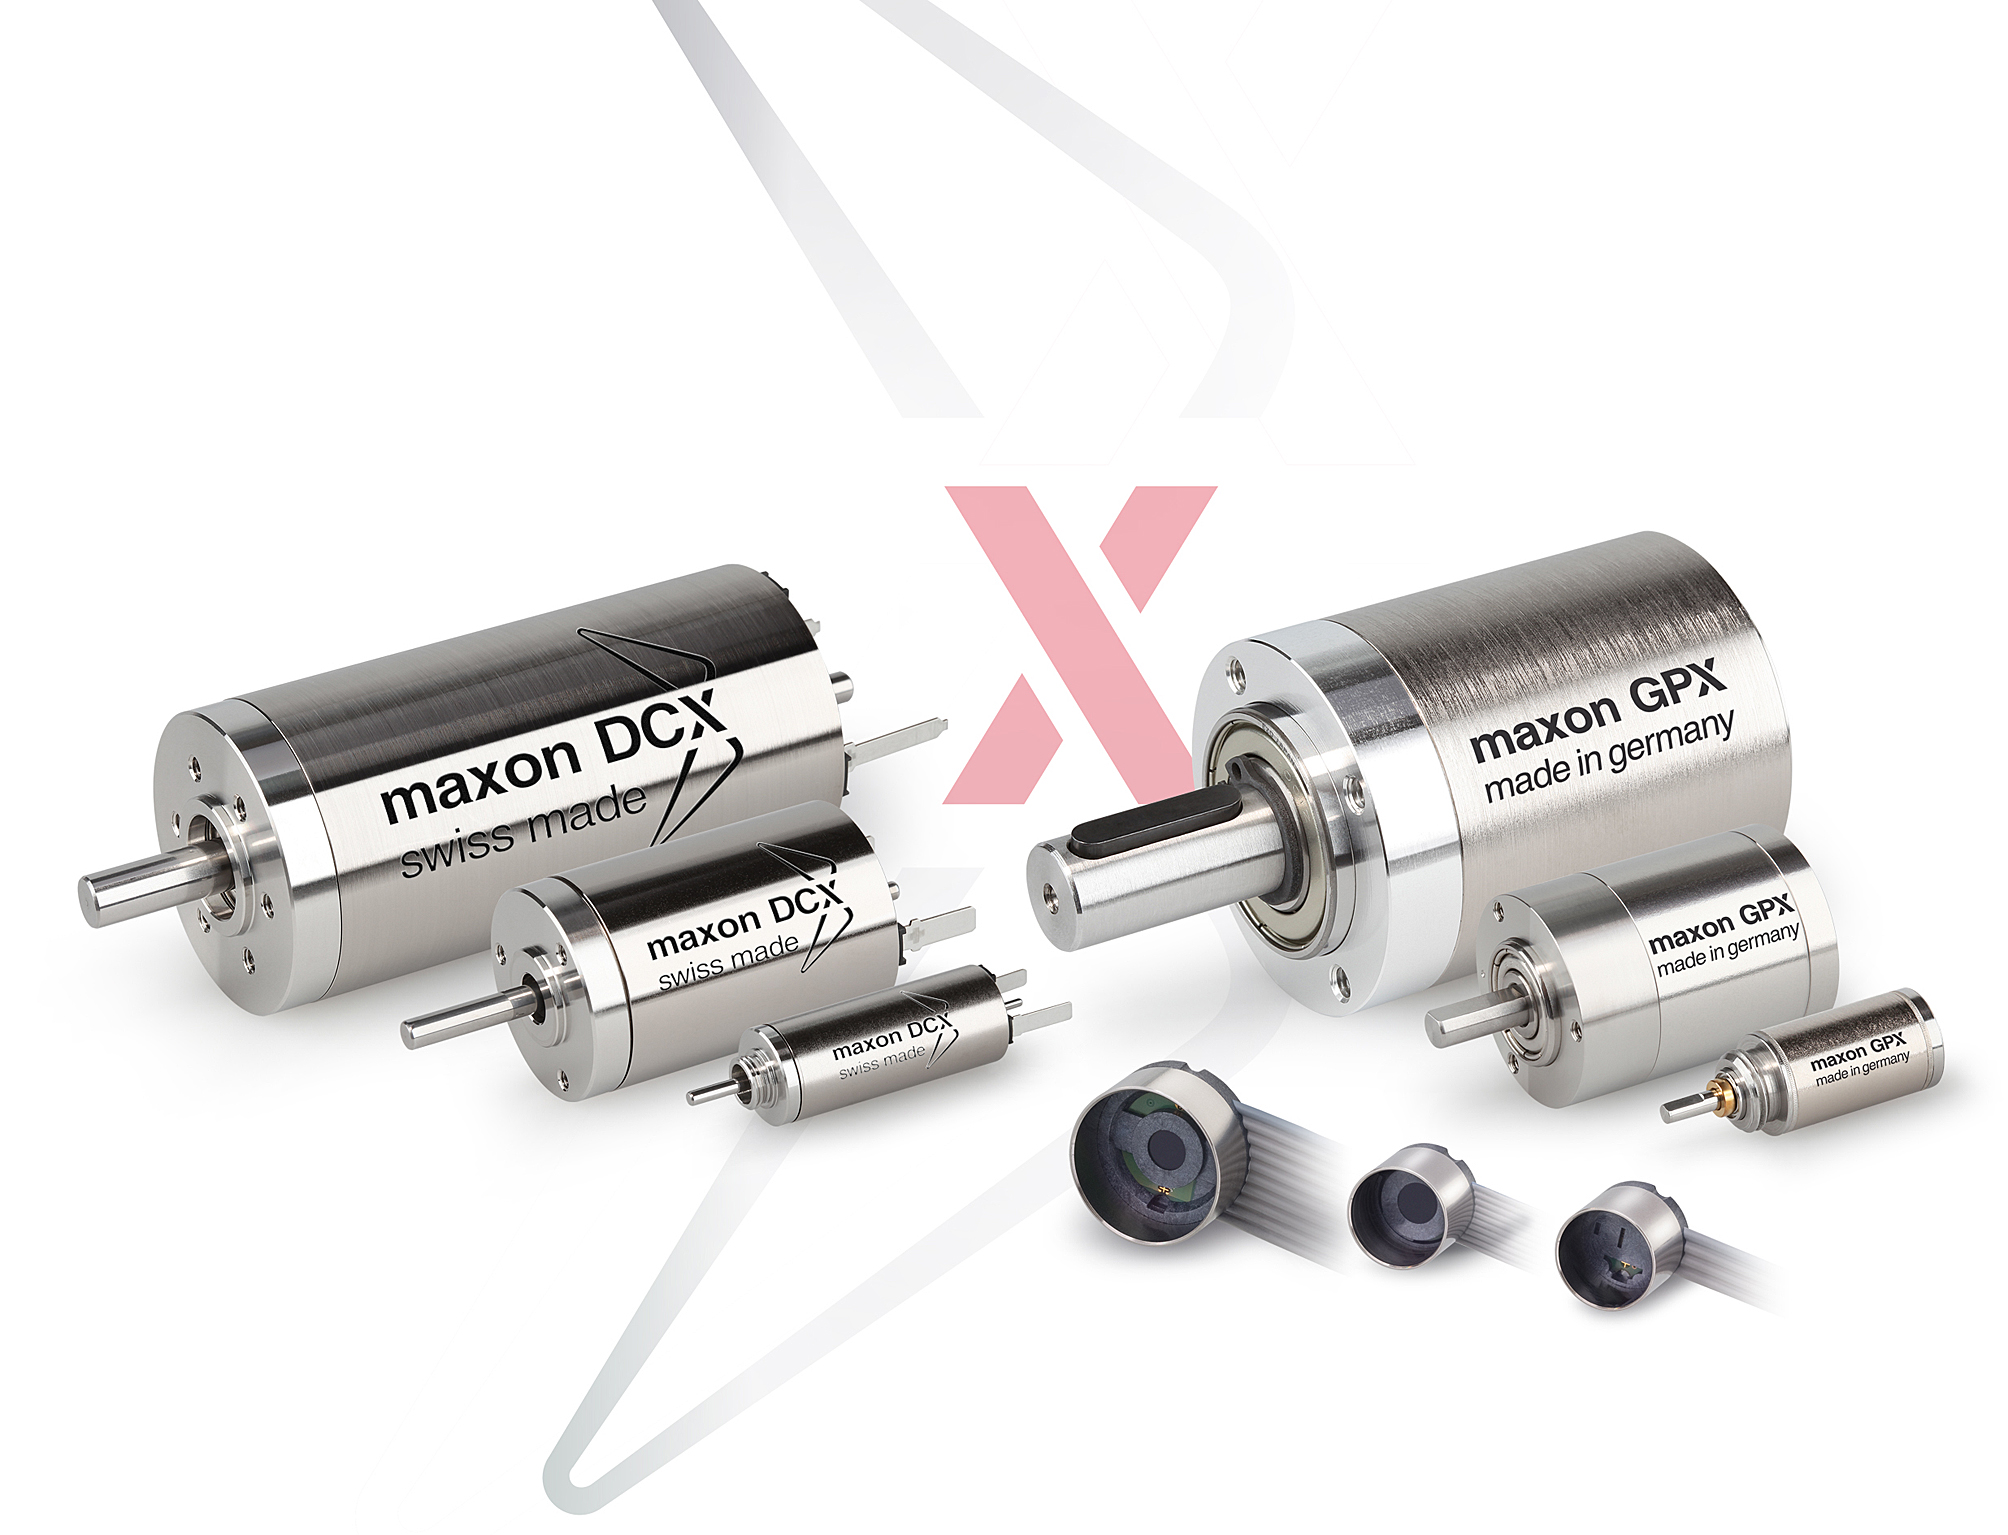
\includegraphics[width=0.8\textwidth]{Kran/Motors.JPG}
        \caption {DC Motoren}
    \end{figure}

%Ablauf
Produktbeschreibung des Funktionsmusters
- Übersichtszeichnungen / Übersichtsmodell
- Beschreibung der Komponenten
- Ablaufdiagramme, Blockdiagramme
- Beschreibung der Funktionalität der einzelnen Blöcke und deren Beziehungen
- Schnittstellenbeschreibungen
- Softwaresubsysteme
- Wichtige Berechnungen (Resultate)
- Beschreibung von Versuchen und Tests mit Ergebnissen 


\end{document}

